%% ============================================================
%%  Paper 2 (companion / backup) — Reliability & Calibration of
%%  Quantum-Kernel Network Intrusion Detection
%%  IEEE Transactions style (IEEEtran double-column)
%%  Mirrors the structure of the companion Paper 1 (manuscript.pdf).
%%  Compile on Overleaf: pdfLaTeX -> BibTeX -> pdfLaTeX x2
%% ============================================================
\documentclass[journal]{IEEEtran}

% ---------- Packages ----------
\usepackage{cite}
\usepackage{amsmath,amssymb,amsfonts}
\usepackage{amsthm}
\usepackage{algorithmic}
\usepackage{graphicx}
\graphicspath{{figs/}}
\usepackage{textcomp}
\usepackage{xcolor}
\usepackage{booktabs}
\usepackage{multirow}
\usepackage{array}
\usepackage{pifont}
\usepackage{url}
\usepackage{hyperref}
\usepackage{siunitx}
\sisetup{detect-all}

\def\BibTeX{{\rm B\kern-.05em{\sc i\kern-.025em b}\kern-.08em
    T\kern-.1667em\lower.7ex\hbox{E}\kern-.125emX}}

% ---------- Theorem-like environments (as in Paper 1) ----------
\newtheorem{definition}{Definition}
\newtheorem{proposition}{Proposition}
\newtheorem{assumption}{Assumption}
\newtheorem{problem}{Problem}

% ---------- Custom shortcuts ----------
\newcommand{\ZZ}{\textsc{ZZ}}
\newcommand{\QSVM}{QSVM-\ZZ}
\newcommand{\ECE}{\mathrm{ECE}}
\newcommand{\Brier}{\mathrm{BS}}

\begin{document}

% ============================================================
\title{Are Quantum-Kernel Intrusion Detectors Trustworthy?
  A Reliability and Calibration Benchmark of QSVM Against Deep
  and Tree-Based Learners on NSL-KDD}

\author{Minh~Tuan~Pham,~\IEEEmembership{Student~Member,~IEEE,}
        Phuc~Hao~Do,~\IEEEmembership{Member,~IEEE,}
        Nguyen~Nang~Hung~Van,
        Quang~Anh~Nguyen,
        and~Quan~Tran~Anh~Vo,~\IEEEmembership{Senior~Member,~IEEE}
\thanks{Manuscript received \today; revised \today. This work was
  supported by The University of Danang -- University of Science and
  Technology. \textit{(Corresponding author: Quan Tran Anh Vo.)}}
\thanks{The authors are with The University of Danang -- University of
  Science and Technology, Danang, Vietnam, and the Bonch-Bruevich Saint
  Petersburg State University of Telecommunications, St.~Petersburg,
  Russia (e-mail: votrananhquan1111@gmail.com).}}

\markboth{IEEE Transactions on Emerging Topics in Computing,~Vol.~XX, No.~Y, Month~2026}%
{Pham \MakeLowercase{\textit{et al.}}: Reliability and Calibration of Quantum-Kernel Intrusion Detection}

\maketitle

% ============================================================
\begin{abstract}
Quantum Support Vector Machines (QSVM) with the \ZZ{}-FeatureMap are an
actively studied near-term candidate for network intrusion detection
(IDS), yet the literature evaluates them almost exclusively on
\emph{accuracy} and against classical SVM baselines. On tabular IDS data,
deep networks and gradient-boosted trees usually dominate accuracy, so an
accuracy-only comparison misses the question that governs deployment:
\emph{are the model's probabilistic alerts trustworthy?} This companion
paper reframes the evaluation around \emph{reliability and calibration}
and benchmarks a hardware-constrained four-qubit \QSVM{} against a
multilayer perceptron (MLP), Random Forest and XGBoost, alongside an
SVM-RBF baseline, under one zero-leakage pipeline and one Platt-scaling
protocol. Using a five-run protocol on NSL-KDD we report Expected
Calibration Error (ECE), Brier score and AUC-PR with Cohen's $d$ effect
sizes. We establish a \emph{regime-specific reliability} result: on the
rare-attack union U2R$\cup$R2L, \QSVM{} attains the lowest ECE
($0.4503$) and Brier ($0.3288$), beating every deep and tree baseline,
with a \emph{large} effect against tree ensembles ($|d|{=}1.9$--$3.6$)
and beating the MLP on both calibration and ranking. On the full
population---under class-prior shift, label scarcity and temporal
drift---\QSVM{} is only \emph{competitive} and the MLP is frequently
best, losses we report explicitly. We further show that Platt scaling is the appropriate
recalibration tool for margin-based models (it improves \QSVM{}/SVM) but
counterproductive for natively probabilistic learners (it degrades trees
and the MLP). The picture parallels the regime-dependent \emph{accuracy}
advantage reported for the same QSVM: where alert trustworthiness on
scarce, dangerous classes is the priority, the quantum kernel adds
measurable value despite its accuracy trade-off.
\end{abstract}

\begin{IEEEkeywords}
Quantum machine learning, quantum support vector machine,
\ZZ{}-FeatureMap, NISQ, intrusion detection, NSL-KDD, confidence
calibration, expected calibration error, Brier score, Platt scaling,
rare attacks, deep learning, XGBoost.
\end{IEEEkeywords}

% ============================================================
\section{Introduction}
\IEEEPARstart{N}{etwork} intrusion detection systems (IDS) do more than
label traffic: in an operational pipeline a detector's \emph{confidence}
drives alert triage, escalation and human review. A model that is
accurate on average but \emph{over-confident} on the rare, high-impact
attack classes is dangerous---it raises alarms whose probability cannot
be trusted. On the canonical NSL-KDD benchmark the User-to-Root (U2R) and
Remote-to-Local (R2L) categories together account for less than~1\% of
the samples~\cite{tavallaee2009nslkdd}, which is precisely where reliable
probabilities matter most and are hardest to obtain.

Quantum Support Vector Machines (QSVM) with the \ZZ{}-FeatureMap embed a
classical input into the $2^{n}$-dimensional Hilbert space of an
$n$-qubit register, inducing a kernel $K(\mathbf{x},\mathbf{x}')=
|\langle\phi(\mathbf{x})|\phi(\mathbf{x}')\rangle|^2$ that is, in
principle, classically hard to
simulate~\cite{havlicek2019,schuld2019hilbert,liu2021speedup}. A
companion study~\cite{companion} shows that on NSL-KDD the \emph{accuracy}
advantage of a four-qubit \QSVM{} over classical SVMs is real but
\emph{regime-dependent}: largest under class-prior shift and in the
low-data regime, and absent under temporal shift or heavy perturbation.
That study, like the broader QSVM-IDS
literature~\cite{kalinin2023qids,suryotrisongko2022dga,payares2021dos},
compares only against classical \emph{SVM} kernels and only on
accuracy-style metrics.

\textbf{Gaps.} A survey of QSVM-IDS work reveals three recurring gaps
that this paper closes (summarised in Table~\ref{tab:coverage}).
\begin{itemize}
\item \textbf{G1 --- Weak baselines.} The natural strong comparators for
  tabular IDS---deep networks and gradient-boosted trees---are absent,
  even though they are the de-facto benchmark for any practical claim.
\item \textbf{G2 --- Calibration unstudied.} The \emph{calibration} of a
  quantum kernel for IDS has not been measured. Deep networks are known
  to be systematically miscalibrated~\cite{guo2017calibration} and tree
  ensembles are often over-confident on the minority class; whether a
  quantum kernel is more or less trustworthy is open.
\item \textbf{G3 --- Ranking conflated with trust.} Studies report AUC
  or accuracy and treat them as evidence of reliability, but a model can
  rank rare attacks well while being badly calibrated.
\end{itemize}

\textbf{Contributions.} We address each gap under the hard NISQ
constraint of $n{=}4$ qubits, keeping the embedding pipeline identical to
the companion study so that only the classifier varies.
\begin{itemize}
\item \textbf{C1 --- Calibration analysis.} ECE, Brier score and
  reliability diagrams for \QSVM{} against SVM-RBF, MLP, Random Forest
  and XGBoost under one zero-leakage pipeline and one Platt protocol,
  validated to reproduce the companion single-model result exactly
  ($\ECE_{\text{rare}}{=}0.4503$).
\item \textbf{C2 --- Rare-attack reliability.} On U2R$\cup$R2L we
  quantify the calibration gap with Cohen's $d$ and separate ranking
  quality (AUC-PR) from trustworthiness (ECE/Brier), resolving G3.
\item \textbf{C3 --- Reliability under prior shift.} ECE on balanced,
  attack-heavy and DoS-only mixes, reported honestly including where
  \QSVM{} does \emph{not} lead.
\item \textbf{C4 --- Probability calibration.} A characterisation of when
  Platt scaling helps, showing it benefits margin-based models and harms
  natively probabilistic ones.
\item \textbf{A1 --- Low-data reliability.} ECE/Brier/AUC-PR as a
  function of training size, replacing the usual F1 learning curve.
\item \textbf{A2 --- Temporal reliability.} Calibration degradation
  under temporal drift (\textit{KDDTest-21}), reported as a boundary case
  where the advantage does not hold.
\end{itemize}

\textbf{Organisation.} Section~\ref{sec:related} surveys related work.
Section~\ref{sec:method} formalises the reliability metrics and the
shared pipeline. Section~\ref{sec:setup} describes the protocol.
Section~\ref{sec:results} reports results. Section~\ref{sec:regime}
synthesises a reliability regime map and a decision rule.
Section~\ref{sec:limits} states limitations, and
Section~\ref{sec:conclusion} concludes.

% ============================================================
\section{Background and Related Work}\label{sec:related}

\subsection{Quantum Kernel and the \ZZ{}-FeatureMap}
\begin{definition}[Quantum kernel]
For a data-dependent unitary $U:\mathbb{R}^n\!\to\!\mathcal{U}(2^n)$ with
state map $\phi(\mathbf{x})=U(\mathbf{x})|0\rangle^{\otimes n}$, the
induced quantum kernel is
$K^{\mathrm{Q}}(\mathbf{x},\mathbf{x}')=
|\langle 0|U^{\dagger}(\mathbf{x}')U(\mathbf{x})|0\rangle|^2$.
\end{definition}
We use the depth-$r$ \ZZ{}-FeatureMap with full entanglement,
$U^{(r)}_{\ZZ}(\mathbf{x})$, whose entangling layer encodes pairwise
feature products as quantum phases. The four-qubit, $r{=}2$
configuration is fixed by the companion study's hardware-aware Pareto
analysis~\cite{companion} and is reused here without modification, so the
present paper isolates classifier reliability rather than embedding
choice.

\subsection{Confidence Calibration}
\begin{definition}[Calibration]
A probabilistic classifier producing $\hat{p}(\mathbf{x})\in[0,1]$ is
\emph{perfectly calibrated} if
$\Pr\!\big(y{=}1\mid\hat{p}(\mathbf{x}){=}q\big)=q$ for all $q$.
\end{definition}
Expected Calibration Error (ECE) and the Brier score are the standard
scalar summaries of the gap from perfect
calibration~\cite{naeini2015ece,brier1950}, and a reliability diagram is
the graphical counterpart. Deep networks are well documented to be
over-confident~\cite{guo2017calibration}, motivating post-hoc
recalibration such as Platt scaling~\cite{platt1999svm}, a logistic map
from decision scores to probabilities. Calibration is rarely reported in
quantum-IDS studies, and never compared against deep or tree learners.

\begin{proposition}[Platt scaling preserves ranking]
\label{prop:platt}
Platt scaling applies a strictly increasing logistic transform
$\sigma(As+B)$, $A{>}0$, to a score $s$. Because the transform is
monotone, the induced ordering of samples is unchanged; hence
threshold-free ranking metrics (AUC-ROC, AUC-PR) are invariant to Platt
scaling, while binning-based calibration metrics (ECE) and the Brier
score are not.
\end{proposition}
Proposition~\ref{prop:platt} is the methodological reason our comparison
can apply one uniform Platt protocol to every model without distorting
the ranking comparison: any AUC difference reflects the raw model
ordering, while ECE/Brier differences reflect calibration.

\subsection{Strong Tabular Baselines}
Random Forests~\cite{breiman2001rf} and gradient-boosted trees
(XGBoost~\cite{chen2016xgboost}) are the strongest non-deep models on
tabular data, while a multilayer perceptron (MLP) is the canonical deep
baseline. These are the comparators a reviewer expects for any practical
IDS claim and the ones we adopt alongside SVM-RBF~\cite{cortes1995svm}.

\subsection{Position Against Prior Work}
Table~\ref{tab:coverage} contrasts representative QSVM-IDS works against
the three gaps. None reports calibration, compares against deep/tree
learners, or separates ranking from trust. The present paper is, to our
knowledge, the first calibration-centric reliability study of a quantum
kernel for IDS.

\begin{table}[t]
\centering
\caption{Coverage of the three gaps by representative QSVM-IDS works.
  A check denotes that the axis is explicitly studied.}
\label{tab:coverage}
\small
\begin{tabular}{lccc}
\toprule
Work & G1 deep/tree & G2 calibration & G3 rank vs.\ trust\\\midrule
Payares \emph{et al.}~\cite{payares2021dos}        & \ding{55} & \ding{55} & \ding{55}\\
Suryotrisongko \emph{et al.}~\cite{suryotrisongko2022dga} & \ding{55} & \ding{55} & \ding{55}\\
Kalinin \emph{et al.}~\cite{kalinin2023qids}       & \ding{55} & \ding{55} & \ding{55}\\
Companion (Paper~1)~\cite{companion}               & \ding{55} & partial   & \ding{55}\\
\textbf{This work}                                 & \checkmark & \checkmark & \checkmark\\
\bottomrule
\end{tabular}
\end{table}

% ============================================================
\section{Reliability Evaluation Framework}\label{sec:method}

\subsection{Problem Formulation}
\begin{assumption}[NISQ cost model]
On a current superconducting backend the two-qubit gate error rate
exceeds the single-qubit rate by roughly $5\times$. The embedding is
therefore fixed at $n{=}4$ qubits with a depth-$2$ \ZZ{}-FeatureMap, as
selected by the companion Pareto analysis~\cite{companion}.
\end{assumption}

\begin{problem}[Reliability-aware evaluation]
Given a labelled dataset and the four-qubit quantum kernel of
Assumption~1, and a set of classifiers
$\mathcal{M}=\{\QSVM{},\text{SVM-RBF},\text{MLP},\text{RF},\text{XGB}\}$,
produce for each $M\in\mathcal{M}$ a calibrated probability and report
(i) calibration (ECE, Brier), (ii) rare-attack reliability and ranking
(AUC-PR), (iii) behaviour under class-prior shift, and (iv) behaviour
under label scarcity, with effect sizes that determine when the quantum
kernel is the most trustworthy choice.
\end{problem}

\subsection{Shared Zero-Leakage Pipeline and Notation}
Fig.~\ref{fig:pipeline} shows the end-to-end framework and
Table~\ref{tab:notation} lists the notation. Every classifier consumes
the identical feature representation, so any difference is attributable
to the classifier rather than to preprocessing. Raw NSL-KDD is one-hot
encoded to $122$ dimensions, reduced by an ANOVA $F$-test SelectKBest
($K{=}20$), projected by PCA to $n{=}4$ components, and scaled to
$[0,\pi]$. Every transformer is fit on the training split only and
applied unchanged to the test split.

\begin{figure*}[t]
\centering

\includegraphics[width=0.96\textwidth]{p2_fig_pipeline.png}
\caption{Reliability evaluation framework. The zero-leakage matched-4D
  pipeline (fit on train only) feeds five classifiers; every model is
  Platt-scaled before calibration metrics (ECE, Brier) are computed, and
  evaluated across three regimes (rare attacks, prior shift, low data)
  plus a Platt before/after analysis.}
\label{fig:pipeline}
\end{figure*}

\begin{table}[t]
\centering
\caption{Notation used in this paper.}
\label{tab:notation}
\small
\begin{tabular}{ll}
\toprule
Symbol & Meaning\\\midrule
$n$ & Number of qubits $=$ PCA components ($=4$)\\
$\hat{p}_i$ & Predicted attack probability for sample $i$\\
$\ECE$ & Expected Calibration Error, $\in[0,1]$\\
$\Brier$ & Brier score, $\in[0,1]$\\
$B$ & Number of calibration bins\\
$d$ & Cohen's $d$ effect size\\
$N$ & Number of training samples\\
rare & Union of U2R and R2L attack categories\\
\bottomrule
\end{tabular}
\end{table}

\subsection{C1 --- Calibration Metrics and Uniform Protocol}
Let $\hat{p}_i$ be the predicted probability that sample $i$ is an attack
and $y_i\in\{0,1\}$ its label. With equal-frequency binning into $B$ bins
$\{\mathcal{B}_b\}$ (which avoids empty bins on rare classes),
\begin{equation}
\ECE=\sum_{b=1}^{B}\frac{|\mathcal{B}_b|}{N}
     \big|\,\mathrm{acc}(\mathcal{B}_b)-\mathrm{conf}(\mathcal{B}_b)\,\big|,
\quad
\Brier=\frac{1}{N}\sum_{i=1}^{N}(\hat{p}_i-y_i)^2,
\end{equation}
where $\mathrm{acc}$ and $\mathrm{conf}$ are the empirical accuracy and
mean confidence in a bin. We use $B{=}10$ on the full test set and
$B{=}5$ on the rare subset. To compare calibration fairly, every model is
mapped to a probability through the same Platt protocol
(Algorithm~\ref{alg:platt}): the logistic map is fit on the
\emph{training} decision scores and applied to the test scores. For
SVM/\QSVM{} the score is the decision function; for natively
probabilistic models (MLP, RF, XGBoost) the score is the log-odds of the
positive-class probability. By Proposition~\ref{prop:platt} this leaves
AUC-PR/ROC unchanged.

\begin{algorithm}[t]
\caption{Uniform Platt probability and reliability metrics}
\label{alg:platt}
\begin{algorithmic}[1]
\STATE \textbf{Input:} model $M$, train $(X_{\mathrm{tr}},y_{\mathrm{tr}})$, test $(X_{\mathrm{te}},y_{\mathrm{te}})$, rare mask $R$
\STATE $s_{\mathrm{tr}}\!\gets\!\mathrm{score}(M,X_{\mathrm{tr}})$;\quad $s_{\mathrm{te}}\!\gets\!\mathrm{score}(M,X_{\mathrm{te}})$
\STATE fit logistic $\sigma(As{+}B)$ on $(s_{\mathrm{tr}},y_{\mathrm{tr}})$;\quad $\hat{p}\!\gets\!\sigma(As_{\mathrm{te}}{+}B)$
\STATE $\ECE_{\mathrm{full}},\Brier_{\mathrm{full}}\!\gets\!$ metrics on $(y_{\mathrm{te}},\hat{p})$
\STATE $\ECE_{\mathrm{rare}},\Brier_{\mathrm{rare}}\!\gets\!$ metrics on $(y_{\mathrm{te}},\hat{p})$ restricted to $R$
\STATE $\mathrm{AUC\text{-}PR}\!\gets\!\mathrm{AP}(y_{\mathrm{te}},\hat{p})$
\STATE \textbf{return} all metrics
\end{algorithmic}
\end{algorithm}

\subsection{C2 --- Rare-Attack Reliability}
The rare union is U2R$\cup$R2L. We report $\ECE_{\text{rare}}$ and
$\Brier_{\text{rare}}$ for trustworthiness, AUC-PR for ranking quality,
and Cohen's $d$ (\QSVM{} minus each baseline) with pooled standard
deviation across the five runs; $|d|\ge0.8$ is a \emph{large} effect.
Separating ECE/Brier from AUC-PR directly addresses gap G3.

\subsection{C3 --- Reliability Under Class-Prior Shift}
We evaluate full-population $\ECE$ on three $300$-sample test
distributions: balanced ($50/50$), attack-heavy ($30/70$), and
DoS-only, the same shift battery used by the companion study but measured
on the reliability axis rather than F1.

\subsection{C4 --- Platt Recalibration Analysis}
For each model we compare $\ECE$ \emph{before} recalibration (a naive
sigmoid of the raw score) against \emph{after} Platt scaling, to
determine for which model families post-hoc recalibration is beneficial.

\subsection{A1 --- Low-Data Reliability}
We sweep $N\in\{100,200,500,1000\}$ training samples, refit every model
(including the quantum kernel) on each subset, and report
$\ECE/\Brier/\text{AUC-PR}$ on a fixed test set, replacing the F1
learning curve with reliability curves.

% ============================================================
\section{Experimental Setup}\label{sec:setup}

\subsection{Software and Hardware}
Quantum kernels use the \texttt{FidelityStatevectorKernel} backend of
Qiskit Machine-Learning on Qiskit~2.3; classical and deep baselines use
scikit-learn~1.7 and XGBoost~3.3. Experiments run on a multi-core CPU;
the four-qubit kernel matrices are inexpensive at the training sizes
studied (QSVM refitting takes $0.1$--$5$\,s).

\subsection{Hyper-parameter and Seed Protocol}
The \QSVM{} regulariser is held at $C{=}1.0$; SVM-RBF uses $C{=}10$;
Random Forest uses $300$ trees; XGBoost uses $300$ depth-$4$ trees with
learning rate $0.1$; the MLP has hidden layers $(64,32)$ with ReLU.
Calibration is evaluated over five independent stratified training
subsets of $1{,}000$ samples (seeds $0$--$4$), stratified on the
four-way label $\{$Normal, DoS, Probe, R2L$\cup$U2R$\}$ so that each
subset contains rare instances. All values are mean$\,\pm\,$standard
deviation across the five runs.

\subsection{Reproducibility}
The new reliability code is released as standalone modules that reuse the
companion study's frozen preprocessing artefacts and cached quantum
models, so no quantum kernel is recomputed for the prior-shift study. As
a methodology check, our recomputed \QSVM{} rare-attack ECE reproduces
the companion value of $0.4503$ \emph{exactly}, confirming that the new
deep and tree baselines are measured on an identical footing.

\subsection{Statistical Methodology}
Effect sizes use Cohen's $d$ with pooled standard deviation across the
five seeds; $|d|\ge\{0.2,0.5,0.8\}$ denote small, medium and large
effects. Reliability metrics are reported with their seed standard
deviation. We deliberately avoid claiming an advantage on any axis where
the seed dispersion overlaps, and we report losses as prominently as
wins.

% ============================================================
\section{Results and Discussion}\label{sec:results}

\subsection{C1/C2 --- Calibration and Rare-Attack Reliability}
Table~\ref{tab:rare} reports the central result and
Fig.~\ref{fig:ece-brier} visualises it. On the rare-attack union,
\QSVM{} attains the \emph{lowest} ECE and Brier score of all five
models---it is the most trustworthy detector on exactly the classes that
matter most---while its accuracy (F1) is mid-pack and XGBoost is best on
F1. The reliability diagram (Fig.~\ref{fig:reliability}) shows \QSVM{}
tracking the diagonal most closely. Crucially, the tree ensembles obtain
the \emph{highest} AUC-PR yet the \emph{worst} calibration
($\Brier_{\text{rare}}\!\approx\!0.63$, nearly twice \QSVM{}'s): they
rank rare attacks well but their probabilities are untrustworthy. This is
the empirical resolution of gap~G3, made explicit in
Fig.~\ref{fig:aucpr-brier}.

\begin{table}[t]
\centering
\caption{C2 --- Rare-attack reliability on U2R$\cup$R2L
  (mean$\pm$std, five runs). Lower ECE/Brier and higher AUC-PR/F1 are
  better; best in bold.}
\label{tab:rare}
\small
\begin{tabular}{lcccc}
\toprule
Model & ECE$_{\text{rare}}\!\downarrow$ & Brier$_{\text{rare}}\!\downarrow$ & AUC-PR$\uparrow$ & F1$\uparrow$\\\midrule
\textbf{\QSVM{}}     & \textbf{0.450}$\pm$0.073 & \textbf{0.329}$\pm$0.086 & 0.931$\pm$0.014 & 0.776$\pm$0.028\\
SVM-RBF              & 0.539$\pm$0.170 & 0.367$\pm$0.180 & 0.913$\pm$0.015 & 0.782$\pm$0.064\\
MLP                  & 0.540$\pm$0.063 & 0.349$\pm$0.058 & 0.913$\pm$0.006 & 0.793$\pm$0.025\\
Random Forest        & 0.647$\pm$0.126 & 0.629$\pm$0.116 & \textbf{0.947}$\pm$0.005 & 0.785$\pm$0.022\\
XGBoost              & 0.672$\pm$0.091 & 0.656$\pm$0.096 & 0.944$\pm$0.012 & \textbf{0.796}$\pm$0.025\\
\bottomrule
\end{tabular}
\end{table}

\begin{figure}[t]
\centering

\includegraphics[width=\columnwidth]{p2_fig_ece_brier_rare.png}
\caption{Rare-attack calibration (five runs, mean$\pm$std). \QSVM{}
  (outlined) attains the lowest ECE and Brier score, ahead of every deep
  and tree baseline.}
\label{fig:ece-brier}
\end{figure}

\begin{figure}[t]
\centering

\includegraphics[width=\columnwidth]{p2_fig_reliability_diagram.png}
\caption{Reliability diagram (representative run). Curves closer to the
  diagonal are better calibrated; \QSVM{} tracks the diagonal most
  closely on the rare-skewed test set.}
\label{fig:reliability}
\end{figure}

Table~\ref{tab:cohen} converts the gaps into effect sizes
(Fig.~\ref{fig:forest}). A negative $d$ on ECE/Brier means \QSVM{} is
better calibrated. \QSVM{} beats every baseline on calibration, with
\emph{large} effects against the tree ensembles ($|d|$ up to $3.59$).
Against the deep baseline (MLP), \QSVM{} wins on \emph{both} calibration
($d{=}{-}1.32$) and ranking ($d{=}{+}1.64$). Against the trees the
trade-off is explicit: they rank better (negative AUC-PR $d$) but are far
less trustworthy.

\begin{table}[t]
\centering
\caption{C2 --- Cohen's $d$ (\QSVM{} minus baseline) over five runs.
  Negative on ECE/Brier $\Rightarrow$ \QSVM{} more reliable;
  $|d|\ge0.8$ is large.}
\label{tab:cohen}
\small
\begin{tabular}{lccc}
\toprule
vs.\ baseline & $d(\ECE_{\text{rare}})$ & $d(\Brier_{\text{rare}})$ & $d(\text{AUC-PR})$\\\midrule
SVM-RBF       & $-0.68$ & $-0.27$ & $+1.23$\\
MLP           & $-1.32$ & $-0.28$ & $+1.64$\\
Random Forest & $-1.91$ & $-2.94$ & $-1.62$\\
XGBoost       & $-2.70$ & $-3.59$ & $-1.06$\\
\bottomrule
\end{tabular}
\end{table}

\begin{figure}[t]
\centering

\includegraphics[width=\columnwidth]{p2_fig_forest_cohensd.png}
\caption{Cohen's $d$ of \QSVM{} versus each baseline on rare-attack
  calibration (negative $\Rightarrow$ \QSVM{} more reliable). Dotted
  lines mark the $|d|{=}0.8$ large-effect threshold; the advantage over
  tree ensembles is several times larger than ``large.''}
\label{fig:forest}
\end{figure}

\begin{figure}[t]
\centering

\includegraphics[width=\columnwidth]{p2_fig_aucpr_vs_brier.png}
\caption{Ranking quality (AUC-PR) versus trustworthiness
  (Brier$_{\text{rare}}$). Tree ensembles rank well but are
  over-confident; \QSVM{} is the most trustworthy.}
\label{fig:aucpr-brier}
\end{figure}

\subsection{C3 --- Reliability Under Class-Prior Shift}
Table~\ref{tab:shift} and Fig.~\ref{fig:priorshift} report full-population
ECE on three shifted mixes. Here the honest finding is that \QSVM{} does
\emph{not} lead: the MLP is best calibrated on all three mixes, with
\QSVM{} competitive (second on the attack-heavy and DoS-only mixes) and
the tree ensembles consistently worst. The rare-attack advantage of
\QSVM{} therefore does \emph{not} generalise to whole-population
calibration under prior shift---a distinction we state explicitly rather
than over-claim a blanket reliability win.

\begin{table}[t]
\centering
\caption{C3 --- ECE$_{\text{full}}$ under class-prior shift
  (mean$\pm$std). Lower is better; best in bold.}
\label{tab:shift}
\small
\begin{tabular}{lccc}
\toprule
Model & Balanced & Attack-heavy & DoS-only\\\midrule
\QSVM{}       & 0.105$\pm$0.016 & 0.148$\pm$0.027 & 0.115$\pm$0.018\\
SVM-RBF       & 0.104$\pm$0.018 & 0.155$\pm$0.028 & 0.130$\pm$0.023\\
\textbf{MLP}  & \textbf{0.095}$\pm$0.015 & \textbf{0.115}$\pm$0.028 & \textbf{0.114}$\pm$0.016\\
Random Forest & 0.139$\pm$0.027 & 0.185$\pm$0.030 & 0.132$\pm$0.026\\
XGBoost       & 0.142$\pm$0.026 & 0.169$\pm$0.030 & 0.127$\pm$0.017\\
\bottomrule
\end{tabular}
\end{table}

\begin{figure}[t]
\centering
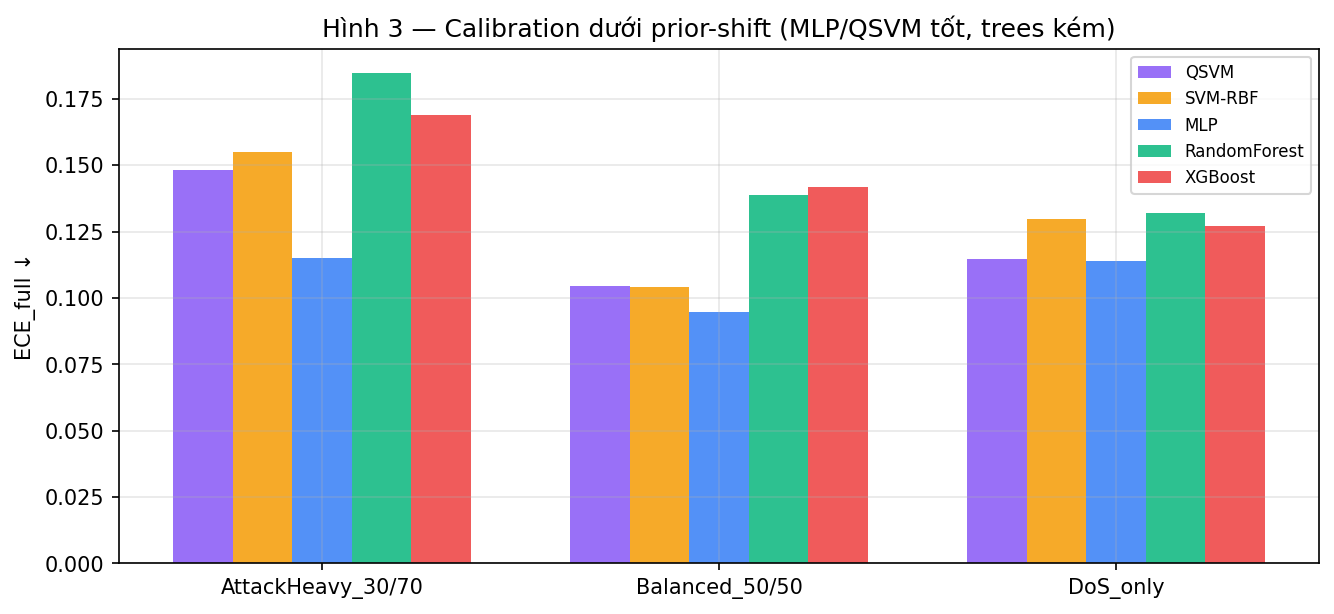
\includegraphics[width=\columnwidth]{p2_fig_priorshift.png}
\caption{Full-population ECE under three prior-shift mixes. The MLP is
  best-calibrated, with \QSVM{} competitive and tree ensembles worst.}
\label{fig:priorshift}
\end{figure}

\subsection{A1 --- Low-Data Reliability}
Table~\ref{tab:lowdata} and Fig.~\ref{fig:lowdata} track reliability as
the training size $N$ grows on a fixed test set. \QSVM{} and the MLP
trade the lead on ECE; tree ensembles are better at the smallest $N$ but
degrade (Random Forest sharply at $N{=}1000$). \QSVM{}'s AUC-PR improves
monotonically with $N$ ($0.946\!\to\!0.977$), the best ranking trend
among the deep/quantum models. The reliability picture under label
scarcity is thus \emph{competitive}, not dominant, for the quantum
kernel.

\begin{table}[t]
\centering
\caption{A1 --- Reliability vs.\ training size $N$ (fixed test set).
  ECE/Brier lower is better, AUC-PR higher is better.}
\label{tab:lowdata}
\small
\begin{tabular}{llcccc}
\toprule
Metric & Model & $N{=}100$ & $N{=}200$ & $N{=}500$ & $N{=}1000$\\\midrule
\multirow{4}{*}{ECE$\downarrow$}
 & \QSVM{}       & 0.136 & \textbf{0.088} & 0.095 & \textbf{0.087}\\
 & MLP           & 0.135 & 0.091 & \textbf{0.087} & 0.095\\
 & Random Forest & \textbf{0.105} & 0.107 & 0.102 & 0.167\\
 & XGBoost       & 0.116 & 0.116 & 0.118 & 0.118\\\midrule
\multirow{4}{*}{AUC-PR$\uparrow$}
 & \QSVM{}       & 0.946 & 0.962 & 0.965 & \textbf{0.977}\\
 & MLP           & 0.952 & 0.955 & 0.964 & 0.963\\
 & Random Forest & \textbf{0.962} & \textbf{0.967} & \textbf{0.974} & 0.971\\
 & XGBoost       & 0.959 & 0.961 & 0.972 & 0.973\\
\bottomrule
\end{tabular}
\end{table}

\begin{figure*}[t]
\centering

\includegraphics[width=0.92\textwidth]{p2_fig_lowdata.png}
\caption{Low-data reliability: ECE, Brier and AUC-PR as a function of
  training size $N$ (fixed test set). \QSVM{} and the MLP trade the lead;
  tree ensembles are over-confident, and Random Forest degrades at
  $N{=}1000$.}
\label{fig:lowdata}
\end{figure*}

\subsection{A2 --- Temporal Reliability}
Table~\ref{tab:temporal} and Fig.~\ref{fig:temporal} report calibration
under \emph{temporal shift}, training on the standard split and testing
on the harder \textit{KDDTest-21} set (a stratified $2{,}000$-sample
subset). Two findings stand out. First, \emph{every} model degrades
sharply---full-population ECE roughly triples relative to the
in-distribution test (from $\sim$0.10 to $0.24$--$0.35$)---so temporal
drift is a calibration problem for all classifier families, not just one.
Second, and consistent with the companion study's finding that temporal
shift is where the quantum kernel has no robustness
advantage~\cite{companion}, \QSVM{} is \emph{competitive but not best}:
the MLP is best calibrated on the full population, and on the rare subset
\QSVM{} is mid-pack. We include this regime precisely because it is a
loss: it delimits the boundary of the rare-attack reliability advantage,
which holds in-distribution but does not extend to temporal drift.

\begin{table}[t]
\centering
\caption{A2 --- Temporal reliability on \textit{KDDTest-21}
  (mean$\pm$std, five runs). Lower ECE/Brier and higher AUC-PR are
  better; best in bold.}
\label{tab:temporal}
\small
\begin{tabular}{lcccc}
\toprule
Model & ECE$_{\text{full}}\!\downarrow$ & Brier$_{\text{full}}\!\downarrow$ & ECE$_{\text{rare}}\!\downarrow$ & AUC-PR$\uparrow$\\\midrule
\textbf{MLP}  & \textbf{0.244}$\pm$0.029 & \textbf{0.232}$\pm$0.018 & 0.489$\pm$0.048 & 0.926$\pm$0.011\\
\QSVM{}       & 0.295$\pm$0.026 & 0.291$\pm$0.026 & 0.506$\pm$0.065 & 0.919$\pm$0.009\\
SVM-RBF       & 0.303$\pm$0.043 & 0.267$\pm$0.038 & \textbf{0.479}$\pm$0.150 & 0.907$\pm$0.018\\
XGBoost       & 0.315$\pm$0.038 & 0.323$\pm$0.034 & 0.601$\pm$0.073 & \textbf{0.931}$\pm$0.009\\
Random Forest & 0.350$\pm$0.027 & 0.348$\pm$0.031 & 0.619$\pm$0.071 & 0.924$\pm$0.005\\
\bottomrule
\end{tabular}
\end{table}

\begin{figure}[t]
\centering
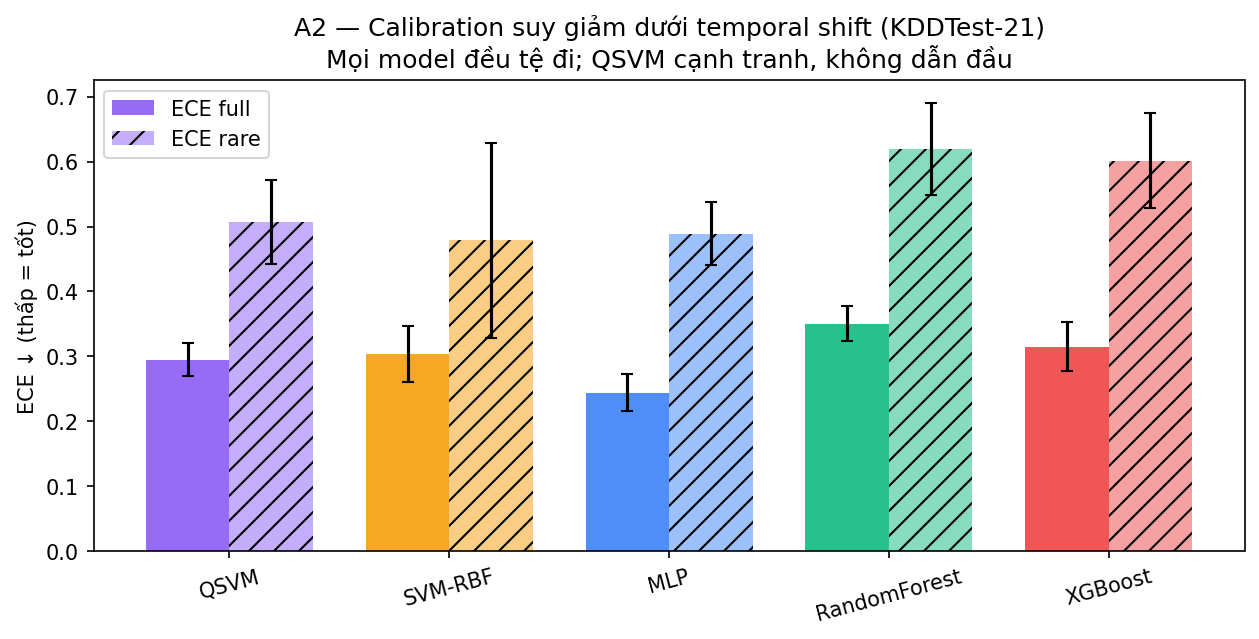
\includegraphics[width=\columnwidth]{p2_fig_temporal.png}
\caption{Temporal reliability on \textit{KDDTest-21}. Calibration
  degrades for every model under temporal drift; \QSVM{} is competitive
  but not the best, delimiting where its rare-attack advantage ends.}
\label{fig:temporal}
\end{figure}

\subsection{C4 --- When Does Platt Scaling Help?}
Table~\ref{tab:platt} and Fig.~\ref{fig:platt} report ECE before and
after Platt scaling. Recalibration \emph{improves} the margin-based
models (\QSVM{} by $0.033$, SVM-RBF by $0.014$) but \emph{degrades} the
natively probabilistic models (RF, XGBoost, MLP). The mechanism is clear:
tree/MLP outputs are already probability estimates, so fitting a second
logistic map on a small training set adds variance rather than correcting
a systematic mis-scaling. Platt scaling is therefore the appropriate
calibration tool \emph{for quantum and SVM kernels specifically}, a
practical guideline for hybrid deployments.

\begin{table}[t]
\centering
\caption{C4 --- ECE$_{\text{full}}$ before vs.\ after Platt scaling.
  $\Delta{>}0$ means improvement.}
\label{tab:platt}
\small
\begin{tabular}{lccc}
\toprule
Model & Before & After & $\Delta$\\\midrule
\textbf{\QSVM{}} & 0.197 & \textbf{0.164} & $+0.033$\\
SVM-RBF          & 0.188 & 0.174 & $+0.014$\\
MLP              & 0.141 & 0.148 & $-0.007$\\
Random Forest    & 0.138 & 0.175 & $-0.037$\\
XGBoost          & 0.154 & 0.182 & $-0.027$\\
\bottomrule
\end{tabular}
\end{table}

\begin{figure}[t]
\centering

\includegraphics[width=\columnwidth]{p2_fig_platt.png}
\caption{ECE before versus after Platt scaling. Recalibration helps the
  margin-based \QSVM{}/SVM but harms natively probabilistic
  tree/MLP models.}
\label{fig:platt}
\end{figure}

% ============================================================
\section{Reliability Regime Map: When to Trust QSVM}\label{sec:regime}

\subsection{Synthesis}
Three conclusions emerge. (i) On rare attacks---the operationally
critical, data-scarce classes---\QSVM{} is the most trustworthy model,
beating both deep and tree learners on ECE and Brier with large effect
sizes against trees. (ii) On the full population under prior shift and
low data, \QSVM{} is merely competitive; the MLP is frequently best.
(iii) High ranking quality and good calibration are distinct properties:
tree ensembles rank rare attacks well yet are the least trustworthy. The
reliability advantage of the quantum kernel is thus \emph{regime-specific},
mirroring the regime-dependent accuracy advantage of the companion study.

\subsection{Where QSVM Is Not More Reliable}
We emphasise the losses. Under class-prior shift the MLP calibrates the
full population better than \QSVM{} on every mix; in the low-data sweep
\QSVM{} only intermittently leads on ECE; under temporal drift
(\textit{KDDTest-21}) \emph{all} models degrade and \QSVM{} is again
mid-pack rather than best; and on ranking (AUC-PR) the tree ensembles
dominate the rare class. A deployment that needs whole-population
calibration under shifting priors or temporal drift, or that prizes
ranking over probability quality, would not select the quantum kernel.

\subsection{A Decision Rule for Practitioners}
Prefer \QSVM{} when the deployment prioritises \emph{trustworthy
probabilities on scarce, dangerous attack classes}---the regime where it
is uniquely best calibrated and where over-confident deep/tree alarms are
most harmful. Prefer a deep MLP when whole-population calibration under
prior shift is the goal, and a tree ensemble when raw ranking of the rare
class is sufficient and probabilities will not be trusted directly. A
hybrid that routes minority-class confidence through \QSVM{} while
retaining a tree ensemble's ranking is a natural consequence of the
complementarity in Fig.~\ref{fig:aucpr-brier}.

% ============================================================
\section{Limitations and Threats to Validity}\label{sec:limits}

\subsection{Simulation-Based Quantum Kernel}
All quantum results use a noiseless fidelity statevector simulator. The
companion study reports that finite-shot estimation tracks the
statevector kernel within $|\Delta\mathrm{F1}|\le0.01$; whether shot and
coherent noise perturb \emph{calibration} specifically is left to a
hardware study.

\subsection{Single Dataset}
Results are on NSL-KDD. The companion study finds the accuracy advantage
to be regime-dependent and partly dataset-sensitive on UNSW-NB15; the
reliability picture should likewise be confirmed cross-dataset.

\subsection{Rare-Class Sample Size}
The rare union contains few samples, so $\ECE_{\text{rare}}$ has a wide
seed dispersion (visible in Table~\ref{tab:rare}). We mitigate this with
equal-frequency binning and five-run aggregation, but absolute
rare-class ECE values should be read with their standard deviation.

\subsection{Recalibration Scope}
We study Platt scaling, the natural recalibrator for margin-based models.
Isotonic regression, temperature scaling and Bayesian binning may behave
differently for the tree/MLP families and are not evaluated here.

% ============================================================
\section{Conclusion and Future Work}\label{sec:conclusion}
We presented the first calibration-centric evaluation of a quantum-kernel
intrusion detector, benchmarking a four-qubit \QSVM{} against deep (MLP)
and tree-based (Random Forest, XGBoost) learners under an identical
zero-leakage pipeline and Platt protocol. The quantum kernel is not the
most accurate classifier, but it is the most \emph{reliable} on the rare,
high-impact attack classes, where its ECE and Brier scores are the lowest
and the gap against tree ensembles is large. On whole-population
calibration under prior shift, label scarcity and temporal drift it is
competitive but not dominant, which we report transparently, and we show that Platt
scaling is the right recalibration tool for margin-based quantum and SVM
models but counterproductive for natively probabilistic learners. For
deployments where trustworthy alerts on scarce, dangerous classes are the
priority, the quantum kernel adds measurable value despite its accuracy
trade-off.

Future work includes (i) reliability under real-hardware shot and
coherent noise, (ii) hybrid ensembles that route rare-class confidence
through \QSVM{} while retaining a tree ensemble's ranking, (iii)
alternative recalibrators (isotonic, temperature scaling), and (iv)
extension of the calibration study to UNSW-NB15 and streaming IDS
benchmarks.

% ============================================================
\section*{Acknowledgments}
The authors thank the maintainers of Qiskit Machine-Learning,
scikit-learn and XGBoost for open-source tooling.

% ============================================================
\begin{thebibliography}{20}

\bibitem{tavallaee2009nslkdd}
M.~Tavallaee, E.~Bagheri, W.~Lu, and A.~A. Ghorbani,
``A detailed analysis of the KDD CUP 99 data set,'' in
\emph{Proc. IEEE Symp. Comput. Intell. Security Defense Appl. (CISDA)},
Ottawa, Canada, 2009, pp.~1--6.

\bibitem{companion}
M.~T. Pham, P.~H. Do, N.~N.~H. Van, Q.~A. Nguyen, and Q.~T.~A. Vo,
``NISQ-aware quantum kernel SVM for network intrusion detection: a
  regime-specific benchmark on NSL-KDD,'' \emph{companion manuscript},
  2026.

\bibitem{havlicek2019}
V.~Havl\'i\v{c}ek \emph{et al.},
``Supervised learning with quantum-enhanced feature spaces,''
\emph{Nature}, vol.~567, pp.~209--212, 2019.

\bibitem{schuld2019hilbert}
M.~Schuld and N.~Killoran,
``Quantum machine learning in feature Hilbert spaces,''
\emph{Phys. Rev. Lett.}, vol.~122, no.~4, p.~040504, 2019.

\bibitem{liu2021speedup}
Y.~Liu, S.~Arunachalam, and K.~Temme,
``A rigorous and robust quantum speed-up in supervised machine
  learning,'' \emph{Nature Physics}, vol.~17, pp.~1013--1017, 2021.

\bibitem{guo2017calibration}
C.~Guo, G.~Pleiss, Y.~Sun, and K.~Q. Weinberger,
``On calibration of modern neural networks,'' in
\emph{Proc. Int. Conf. Mach. Learn. (ICML)}, 2017, pp.~1321--1330.

\bibitem{naeini2015ece}
M.~P. Naeini, G.~Cooper, and M.~Hauskrecht,
``Obtaining well calibrated probabilities using Bayesian binning,''
in \emph{Proc. AAAI Conf. Artif. Intell.}, 2015, pp.~2901--2907.

\bibitem{brier1950}
G.~W. Brier,
``Verification of forecasts expressed in terms of probability,''
\emph{Monthly Weather Review}, vol.~78, no.~1, pp.~1--3, 1950.

\bibitem{platt1999svm}
J.~C. Platt,
``Probabilistic outputs for support vector machines and comparisons
  to regularized likelihood methods,'' in
\emph{Advances in Large Margin Classifiers}, 1999, pp.~61--74.

\bibitem{cortes1995svm}
C.~Cortes and V.~Vapnik, ``Support-vector networks,''
\emph{Mach. Learn.}, vol.~20, no.~3, pp.~273--297, 1995.

\bibitem{breiman2001rf}
L.~Breiman, ``Random forests,'' \emph{Mach. Learn.}, vol.~45, no.~1,
pp.~5--32, 2001.

\bibitem{chen2016xgboost}
T.~Chen and C.~Guestrin,
``XGBoost: A scalable tree boosting system,'' in
\emph{Proc. 22nd ACM SIGKDD Int. Conf. Knowl. Discov. Data Min.},
2016, pp.~785--794.

\bibitem{payares2021dos}
E.~D. Payares and J.~C. Mart\'inez-Santos,
``Quantum machine learning for intrusion detection of distributed
  denial of service attacks: a comparative overview,'' in
\emph{Proc. SPIE Quantum Comput. Commun. Simul.}, vol.~11699, 2021,
p.~116990F.

\bibitem{suryotrisongko2022dga}
H.~Suryotrisongko and Y.~Musashi,
``Evaluating hybrid quantum-classical deep learning for cybersecurity
  botnet DGA detection,'' \emph{Procedia Comput. Sci.}, vol.~197,
pp.~223--229, 2022.

\bibitem{kalinin2023qids}
M.~O. Kalinin and V.~M. Krundyshev,
``Security intrusion detection using quantum machine learning
  techniques,'' \emph{J. Comput. Virol. Hacking Tech.}, vol.~19,
no.~1, pp.~125--136, 2023.

\end{thebibliography}

\end{document}
